\clearpage
\subsection{Affine Varieties} 

\begin{definition}[title = Definition 1.2.1] 
  Let $f_1,\ldots, f_s \in k[x_1, \dots, x_n]$ be finitely many polynomials $(s \in \mathbb{N}_0)$. Then the set $V(f_1, \ldots f_s) = \{(a_1, \ldots, a_n) \in k^n: f_i(a_1, \ldots, a_n) = 0 \forall i = 1, \ldots, s\}$ 
  is called the \textit{affine variety} defined by the polynomials $f_1, \ldots, f_s$. This is the solution set over the field $k$ of the system of polynomial equations.
  \begin{align*}
    \left\{
      \begin{aligned}
          f_1 = 0 \\
          \dots \\ 
          f_s = 0
      \end{aligned}
    \right.
  \end{align*}
 
  To indicate the underlying field explicitly, one also writes $V_k(f_1, \ldots, f_s)$. 
\end{definition}

\begin{example}[title = Example 1.2.2] 
    \begin{minipage}[t]{0.49\textwidth}
     \textbf{1.} $V_{\mathbb{R}}(x^2 + y^2 - 1)$ \\
        \begin{center}
          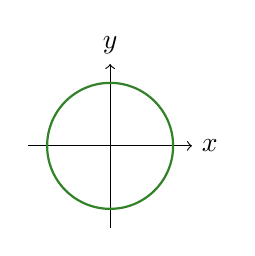
\begin{tikzpicture}[scale=0.8]  

            \draw[->] (-1.3,0) -- (1.3,0) node[right] {$x$};
            \draw[->] (0,-1.3) -- (0,1.3) node[above] {$y$};
                
            \definecolor{kGreen}{RGB}{50,130,40}

              \draw[thick, kGreen] (0,0) circle (1);
          \end{tikzpicture}
        \end{center}
    \end{minipage} 
    \hspace*{0.2cm} 
    \begin{minipage}[t]{0.49\textwidth}
      \textbf{2.} $V_{\mathbb{R}}(y^2-x(x-1)^2)$ \\
        \begin{center}
          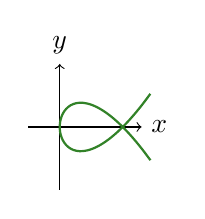
\begin{tikzpicture}[scale=0.8]  

            \draw[->] (-0.5,0) -- (1.3,0) node[right] {$x$};
            \draw[->] (0,-1) -- (0,1) node[above] {$y$};
                
            \definecolor{kGreen}{RGB}{50,130,40}

              \draw[thick, kGreen, domain=-1.2:1.2, samples=50, smooth, variable=\t]
             plot ({\t*\t}, {\t*(\t*\t-1)});
          \end{tikzpicture}
        \end{center}        
          Cubic elliptic curve over $\mathbb{R}$ with a singularity. In cryptography one uses elliptic curves over finite fields \underline{without} singularities for encryption purposes. \\

          \centering{\textcolor{airforceblue}{\textit{Whenever you use firefox you use elliptic curve encryption.}}}
    \end{minipage}
  \vspace{0.5cm}

    \begin{minipage}[t]{0.49\textwidth}
        \textbf{3.} $V_{\mathbb{R}}(z - x^2 - y^2)$ \\ 
        \begin{center}  
        %   \begin{tikzpicture}[scale=0.8]  
        %     \begin{axis}[
        %         xlabel=$x$, ylabel=$y$, zlabel=$z$,
        %         view={135}{30}, axis lines=middle,
        %         xmin=-1.3, xmax=1.3, ymin=-1.3, ymax=1.3, zmin=0, zmax = 1.5,   restrict z to domain=0:2
        %       ]
        %       \addplot3[surf, opacity=0.6, z buffer=sort,
        %       samples=40, samples y=15,
        %       domain=0:360, y domain=0:1]
        %       ({y*cos(x)}, {y*sin(x)}, {y^2});

        %     \end{axis}
        % \end{tikzpicture}  

        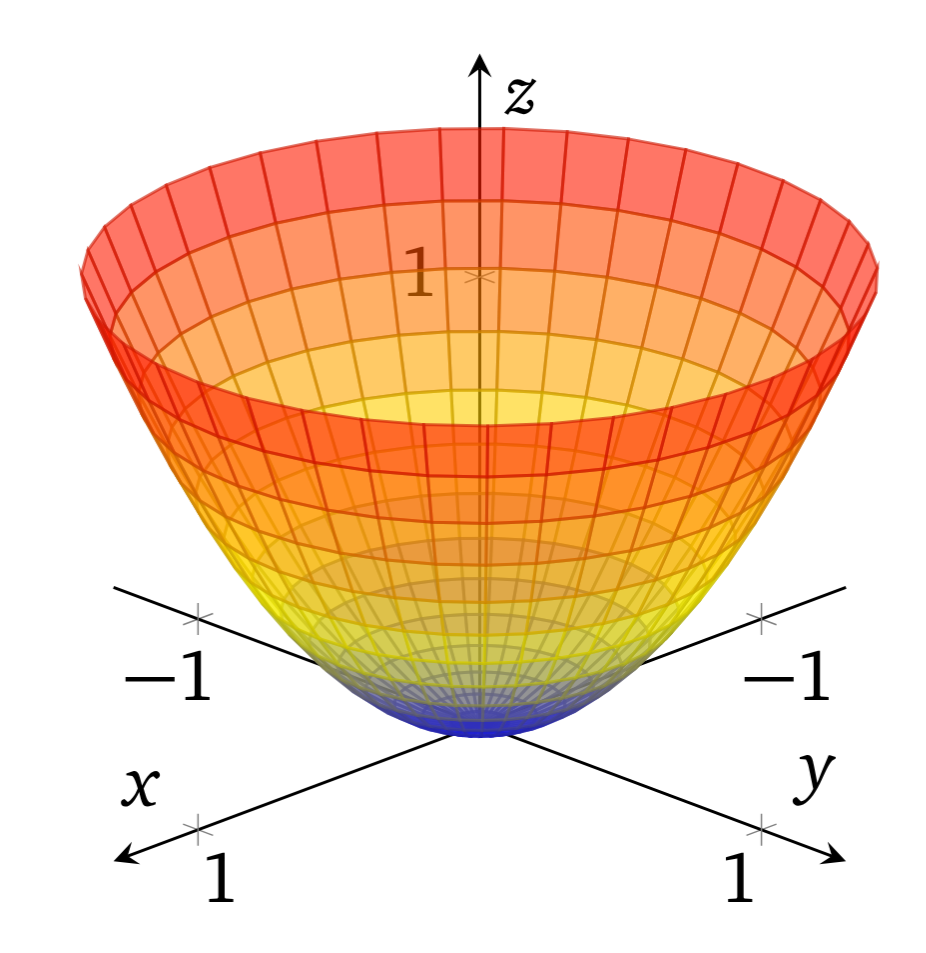
\includegraphics[scale = 0.125]{pics/ex_3.png}
        \end{center}
        Paraboloid
    \end{minipage}
    \hspace*{0.2cm}
    \begin{minipage}[t]{0.49\textwidth}
        \textcolor{airforceblue}{\textit{\textbf{Side Note}: Why is a satelite dish parabolic?}} \\ 
          \begin{center}  
            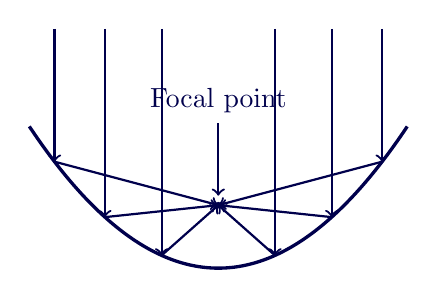
\begin{tikzpicture}[line width=0.8pt, scale = 0.8, color=blue!30!black]
              % Parabolspiegel: y = x^2/(4f) mit f = 1
              \draw[domain=-3:3, samples=60, smooth, line width=1.2pt]
                plot (\x, {\x*\x/4});

              % Einfallende Strahlen und Reflexion zum Brennpunkt
              \foreach \x in {-2.6,-1.8,-0.9,0.9,1.8,2.6} {
                \draw[->] (\x, 3.8) -- (\x, {\x*\x/4});
                \draw[->] ({\x}, {\x*\x/4}) -- (0, 1);
              }

              % Brennpunkt
              \fill (0,1) circle (1.5pt);
              \draw[->] (0,2.3) -- (0,1.15);
              \node[above] at (0,2.3) {Focal point};
            \end{tikzpicture}
          \end{center}
          \textcolor{airforceblue}{\textit{Car lights work the other way around with the light source in the focal point.}}
    \end{minipage}
\vspace{0.5cm} 

  \begin{minipage}[t]{0.49\textwidth}
    \textbf{4.} $V_{\mathbb{R}}(z^2 - x^2 - y^2)$  \\
      \begin{center}
      % \begin{tikzpicture}[scale=0.8]  
      %   \begin{axis}[
      %     xlabel=$x$, ylabel=$y$, zlabel=$z$,
      %     view={135}{30}, axis lines=middle,
      %     xmin=-1.3, xmax=1.3, ymin=-1.3, ymax=1.3,
      %     zmin=-1.3, zmax=1.3,
      %     colormap/hot, point meta min=-1, point meta max=1
      %   ]
      %     % oberer Kegel: z = r
      %     \addplot3[surf, opacity=0.6, z buffer=sort,
      %               samples=40, samples y=10,
      %               domain=0:360, y domain=0:1]
      %       ({y*cos(x)}, {y*sin(x)}, {y});
        
      %     % unterer Kegel: z = -r
      %     \addplot3[surf, opacity=0.6, z buffer=sort,
      %               samples=40, samples y=10,
      %               domain=0:360, y domain=0:1]
      %       ({y*cos(x)}, {y*sin(x)}, {-y});
        
      %   \end{axis}
      % \end{tikzpicture} 

      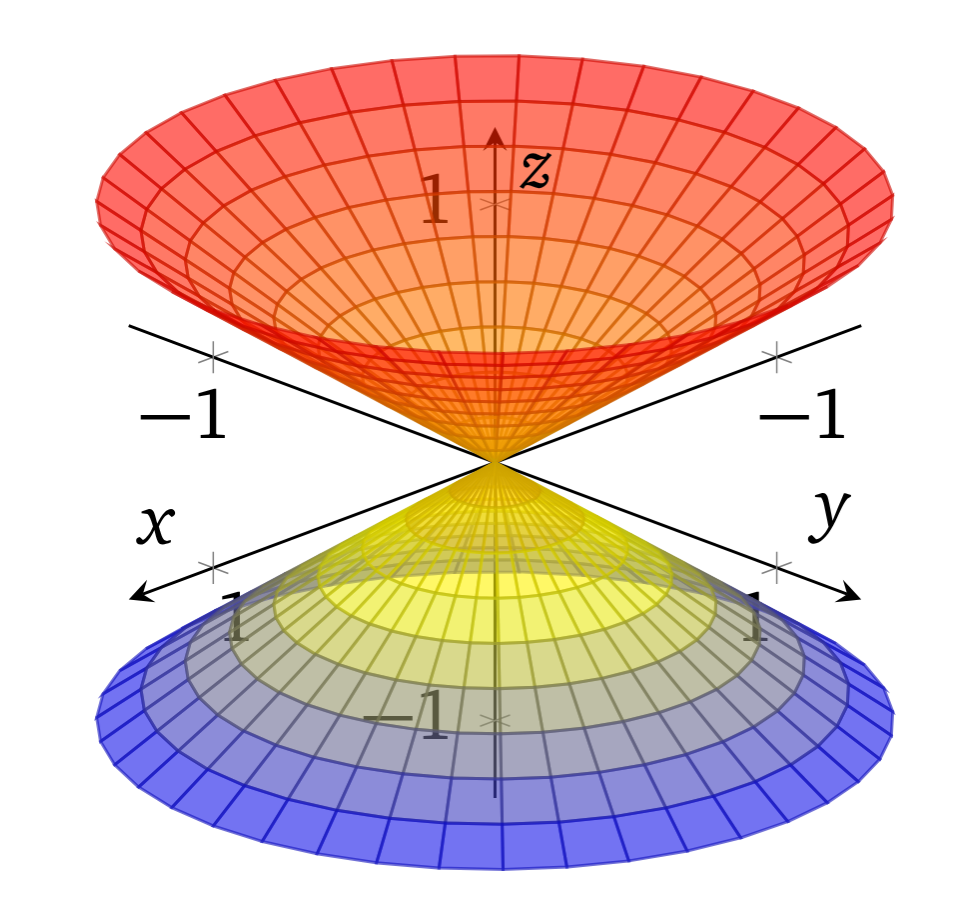
\includegraphics[scale = 0.125]{pics/ex_4.png}
    \end{center}
    Cone 
  \end{minipage}
  \hspace*{0.2cm}
  \begin{minipage}[t]{0.49\textwidth}
    \textbf{5.} $V(x^2 - y^2 \cdot z^2 + z^3)$ \\  
    \begin{center}
        % \begin{tikzpicture}[scale=0.8]  
        %   \begin{axis}[
        %     xlabel=$x$, ylabel=$y$, zlabel=$z$,
        %     view={125}{25}, axis lines=middle,
        %     xmin=-1.6, xmax=1.6, ymin=-1.2, ymax=1.2, zmin=-1, zmax=1.5,
        %     colormap/hot, point meta min=-1, point meta max=1.5
        %   ]
  
        %   \addplot3[surf, opacity=0.7, z buffer=sort, samples=30, samples y=40,
        %             domain=0:1, y domain=-1.2:1.2]
        %     ({(-1+x*(y^2+1))*sqrt(abs(y^2-(-1+x*(y^2+1))))},
        %      {y},
        %      {-1+x*(y^2+1)});

        %   \addplot3[surf, opacity=0.7, z buffer=sort, samples=30, samples y=40,
        %             domain=0:1, y domain=-1.2:1.2]
        %     ({-(-1+x*(y^2+1))*sqrt(abs(y^2-(-1+x*(y^2+1))))},
        %      {y},
        %      {-1+x*(y^2+1)});

        %   \addplot3[thick, kGreen, domain=-1.2:1.2, samples=2] (0,x,0);
        %   \end{axis}
        % \end{tikzpicture} 
        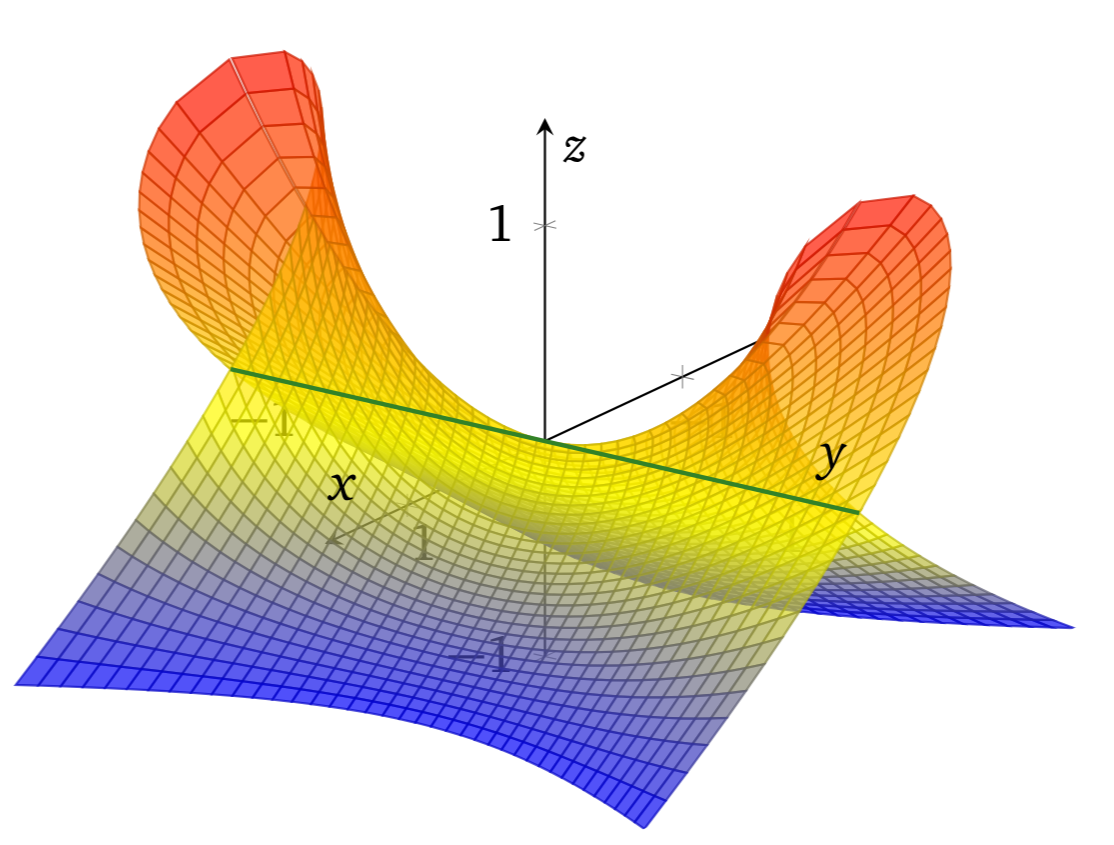
\includegraphics[scale = 0.125]{pics/ex_5.png}
    \end{center} 
  \end{minipage}

\end{example}

\clearpage
 
\begin{example}[title = Example 1.2.2 continued]

  \begin{minipage}[t]{0.49\textwidth}
      \textbf{6.} $V(y-x^2, z - x^3)$
      \begin{center}
  %       \begin{tikzpicture}
  %         \begin{axis}[
  %             view={125}{20},
  %             xlabel=$x$, ylabel=$y$, zlabel=$z$,
  %             xmin=-1.5, xmax=1.5, ymin=0, ymax=2.5, zmin=-3.5, zmax=3.5,
  %             colormap={b}{color=(blue!30) color=(blue!30)},
  %             colormap={r}{color=(red!30) color=(red!30)},
  %             z buffer=sort, samples=30, samples y=2]
          
  %           % Surface 1: y = x^2
  %           \addplot3[surf, colormap name=b, opacity=0.5, draw=blue!50,
  %                     domain=-1.5:1.5, y domain=-3.5:3.5]
  %             ({x}, {x^2}, {y});
          
  %           % Surface 2: z = x^3
  %           \addplot3[surf, colormap name=r, opacity=0.5, draw=red!50,
  %                     domain=-1.5:1.5, y domain=0:2.5]
  %             ({x}, {y}, {x^3});
          
  %           % Intersection: (t, t^2, t^3)
  %           \addplot3[very thick, green!50!black, no markers,
  %                     domain=-1.5:1.5, samples=80, samples y=0]
  %             ({x}, {x^2}, {x^3});
  %         \end{axis}
  %       \end{tikzpicture}
  %     \end{center}

      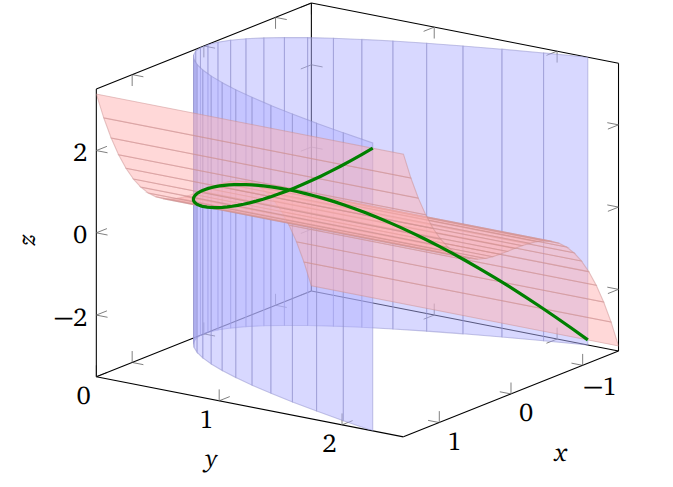
\includegraphics[scale = 0.3]{pics/ex_6.png}
      This is a curve, so called twisted cubic. 
    \end{center}
  \end{minipage} 
  \hspace*{0.2cm}
  \begin{minipage}[t]{0.49\textwidth}
  Linear Case for what happend in 6. 
  \begin{center}
    \begin{tikzpicture}[scale = 0.8]
      \begin{axis}[
        xlabel=$x$, ylabel=$y$, zlabel=$z$,
        view={125}{25}, axis lines=middle,
        xmin=-1.3, xmax=1.3, ymin=-1.3, ymax=1.3, zmin=-1.3, zmax=1.3,
        z buffer=sort,
        colormap={b}{color=(blue!30) color=(blue!30)},
        colormap={r}{color=(red!30) color=(red!30)}
      ]
        % Ebene z = 0
        \addplot3[surf, shader=flat, draw=none, colormap name=b, opacity=0.5,
                  domain=-1.3:1.3, y domain=-1.3:1.3, samples=2]
          {0};

        % Ebene y = 0  (Parametrisierung: x = x, y = 0, z = y)
        \addplot3[surf, shader=flat, draw=none, colormap name=r, opacity=0.5,
                  domain=-1.3:1.3, y domain=-1.3:1.3, samples=2]
          ({x}, {0}, {y});

        % Schnittgerade: x-Achse (y = z = 0)
        \addplot3[very thick, kGreen, no markers,
                  domain=-1.3:1.3, samples=2, samples y=0]
          ({x}, {0}, {0});
      \end{axis}
    \end{tikzpicture} 
  \end{center}
  \end{minipage}
\vspace{0.5cm}

  \begin{minipage}[t]{0.49\textwidth}
    \textbf{7.} $V(xz, yz)$ \\ 
      \begin{center}
      \begin{tikzpicture}[scale = 0.8]
        \begin{axis}[
          xlabel=$x$, ylabel=$y$, zlabel=$z$,
          view={125}{25}, axis lines=middle,
          xmin=-1.3, xmax=1.3, ymin=-1.3, ymax=1.3, zmin=-1.3, zmax=1.3
        ]
          % Ebene z = 0
          \addplot3[surf, shader=flat, draw=none, fill=blue!30, opacity=0.5,
                    z buffer=sort, domain=-1.3:1.3, y domain=-1.3:1.3,
                    samples=2] {0};
        
          % z-Achse (x = y = 0)
          \addplot3[very thick, kGreen, domain=-1.3:1.3, samples=2] (0,0,x);
        \end{axis}
      \end{tikzpicture}
    \end{center}
      This is a union of a line and a plane. \\

      \textbf{8.} $V_{\mathbb{R}}(x^2 + y^2 + 1) = \emptyset$ vs. $V_{\mathbb{C}}(x^2 + y^2 + 1) \neq \emptyset$   \\ 

      \textbf{9.} $V(xy, xy-1) = \empty$ for every field $k$.  \\
      \textbf{Basic Task:} How to figure out, if the variety is empty.

  \end{minipage}
  \hspace*{0.2cm}
  \begin{minipage}[t]{0.49\textwidth}
    \textbf{10.} You can take an algebraic perspective of viewpoint on many topics on math. For example, optimization. Suppose you optimize $f(x, y, z)$ suspect to $g(x,y,z) = 0$ where $f, g \in k[x,y,z]$. \\

    We can do Lagrange multipliers. 
    \begin{align*}
      \left\{ 
      \begin{aligned}
        \frac{\nabla f}{ \nabla x} = \lambda \frac{\nabla g}{\nabla x} \\
        \frac{\nabla f}{ \nabla y} = \lambda \frac{\nabla g}{\nabla y} \\
        \frac{\nabla f}{ \nabla z} = \lambda \frac{\nabla g}{\nabla z} \\
      \end{aligned}
      \right. 
    \end{align*}
    \[\leadsto V(\frac{\nabla f}{\nabla x} - \lambda \frac{\nabla g}{\nabla x}, \frac{\nabla f}{\nabla y} - \lambda \frac{\nabla g}{\nabla y}, \frac{\nabla f}{\nabla z} - \lambda \frac{\nabla g}{\nabla z})\]
    We work in the ring $k[x,y,z, \lambda]$.  
  \end{minipage}     
\vspace{0.5cm}

\begin{minipage}[t]{0.49\textwidth}
  \textbf{11.}  $V(x^2 + y^2 - 4, (x-u)^2 + (y-v)^2 - 1)$ \\ 
  \begin{center}
      \begin{tikzpicture}[
        every node/.style={font=\large}, scale = 0.8,
        vertex/.style={circle, draw=green!40!black, fill=white, inner sep=1.5pt},
        edge/.style={draw=green!40!black, line width=1pt}
      ]
        % Knoten
        \node[vertex, label={[green!40!black]above left:$(x,y)$}] (A) at (0,0) {};
        \node[vertex, label={[green!40!black]right:$(u,v)$}]      (B) at (3,0) {};
        \node[vertex]                                             (C) at (-1,-4) {};

        % Kanten mit Gewichten
        \draw[edge] (A) -- node[above, green!40!black] {$1$} (B);
        \draw[edge] (A) -- node[left,  green!40!black] {$2$} (C);
      \end{tikzpicture}
  \end{center}
  Two-dimensional variety in the space of dimension four. 
\end{minipage}
\hspace*{0.2cm}
\begin{minipage}[t]{0.49\textwidth}
  \textbf{12.} Solution set of linear systems of equations (these are called \textit{affine subspaces}).

\end{minipage}
\end{example}

\clearpage
\begin{center}
    \textcolor{gray}{------------------------------------------- 20.10.2026 --------------------------------------------} \\[0.3em]
\end{center} 
\vspace{0.5cm} 
 
\hspace*{0.5cm}\textcolor{airforceblue}{\textit{(Fix the definition of late to one minute.)}} \\  

\begin{lemma}[title = Lemma 1.2.3]
  Let $V, W \subseteq k^n$ be affine varieties. Then $V \cap W$ and $V \cup W$ are also affine varieties. 

  \paragraph{Proof:} Let $V = V(f_1, \ldots, f_l)$ and $W = V(g_1, \ldots, g_m)$. For finitely many polynomials $f_1, \ldots, f_l, g_1, \ldots, g_l \in k[x_1, \dots, x_n]$. 
  The $V \cap W = V(f_1, \ldots, f_l, g_1, \ldots, g_m)$, so $V \cap W$ is a variety.  

  It turns out that $V \cup W = V(f_i \cdot g_j: i =1, \ldots, l, j = 1, \ldots, m)$.
  Let's varify this. Let $a = (a_1, \ldots, a_n) \in V \cup W$. This means $a \in V$ or $a \in W$. If $a \in V$, then $f_1(a) = f_2(a) = \ldots = f_i(a) = 0$. So, 
  $f_i(a)\cdot g_j(a) = 0$ for all $i$ and $j$. $\Rightarrow$ $a \in V(f_i \cdot g_j: i = 1, \ldots, l, j = 1, \ldots, m)$. 

  For $a \in W$, the argument is analogous. 
  
  To conclude the proof, we consider $a \notin V \cup W$ and show that $a \in V(f_i \cdot g_j: i = 1, \ldots, l, j = 1, \ldots, m)$. 
  Since, $a \notin V\cup W$, we have $a \notin V$ \underline{and} $a \notin W$. Since, $a \notin V$, we have $f_s(a) \neq 0$ for some $s = 1, \ldots, l$. Since, $a \notin W$, 
  we have $g_t(a) \neq 0$ for some $t = 1, \ldots, m$. $\Rightarrow \ f_s(a) \cdot g_t(a) \neq 0 \ \Rightarrow \ a \notin V(f_i \cdot g_j: i = 1, \ldots, l, j = 1, \ldots, m)$   

  \begin{flushright}
    $\Box $
  \end{flushright}

\end{lemma}

\begin{remark}[title = Remark 1.2.3a]
  Any finite subset of $k^n$ is variety. These are so-called zero-dimensional varieties.
\end{remark}

\begin{remark}[title = Remark 1.2.3b]
  Now, you can understand $\underbrace{V(xz, yz)}_{\text{decomposable}} = V(x,y) \cup V(z) \ \leadsto$ irreducible varieties.  
\end{remark}

\begin{remark}[title = Remark 1.2.3c]
  When we were in the kindergarten, we learn linear algebra; the kid whose name was Gauss (smart kid with no friends) told us how to solve things.   \\

  \hspace*{0.5cm}\textcolor{airforceblue}{\textit{(Now we are not in kindergarten anymore, we need to deal with hard life.)}}  \\

  We can ask a few questions about a variety $V = V(f_1, \ldots, f_l)$ for given polynomials $f_1, \ldots, f_l \in k[x_1, \dots, x_n]$. 
  \begin{enumerate}
    \item Is $v \neq 0$, i.e. does the system $f_1 = \ldots = f_l = 0$ have a solution over $k$?  
    \item Is $V$ finite? 
    \item What is the dimension of $V$? (We still need to define dimension and it's not that easy)
  \end{enumerate}
  The hardness of these problems depends on the field. 
\end{remark}

\begin{exercise}[title = Exercise 1.2.4]
  \begin{itemize}
    \item[a)] For the fields you know, decide if they are algebraically closed.  
    \item[b)] For subsets of $k^n$ that you know, decide if they are affine varieties. \\
    Examples: $\mathbb{R}_{\geq 0}$ - is it a variety? , $k \backslash \{0\}$ - is it a variety? 
  \end{itemize}
\end{exercise}

